\begin{frame}
\frametitle{Shopping list: basic hardware for this course}
  \begin{columns}
    \column{0.85\textwidth}
    \begin{itemize}
      \item BeagleBone Black or BeagleBone Black Wireless - Multiple distributors: \\
	    See \url{https://beagleboard.org/Products/}.
      \item 5V power supply, at least 2A, for the BeagleBone Black, with a 5.5 mm barrel
            jack connector. Needed to drive the LCD cape!\\
	    \url{https://www.olimex.com/Products/Power/SY1005E/}
      \item USB Serial Cable - 3.3 V - Female ends (for serial console): \\
	    \url{https://www.olimex.com/Products/Components/Cables/USB-Serial-Cable/USB-SERIAL-F/}
      \item Beagle Bone Black LCD4.3 cape from 4D systems\\
            \url{https://4dsystems.com.au/products/4dcape-43/}
      \item A standard micro SD card - 1 GB or more
      \item A faster micro SD card - 1 GB or more
    \end{itemize}
    \column{0.15\textwidth}
    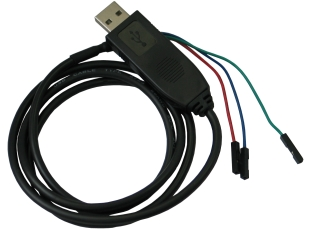
\includegraphics[height=0.20\textheight]{common/usb-serial-cable-female.png} \\
    
\includegraphics[height=0.20\textheight]{common/sd-card.pdf} \\
  \end{columns}
\end{frame}

\begin{frame}
\frametitle{Shopping list: optional hardware for this course}
  If you are interested in doing the optional hardware measurement lab
    \begin{itemize}
      \item A handful of breadboard wires (at least 10 to have sufficient different colors)
	    \footnote{\tiny \url{https://www.olimex.com/Products/Breadboarding/JUMPER-WIRES/JW-110x10/}}
      \item Arduino Nano board (or a clone), with its USB power cable\\
            \url{https://store.arduino.cc/arduino-nano}
      \item A breadboard large enough to plugin the Arduino Nano\\
            \url{https://www.olimex.com/Products/Breadboarding/BREADBOARD-1/}
      \item A four digit display based on the TM1637 chip\\
            \url{https://www.seeedstudio.com/Grove-4-Digit-Display.html}
      \item A 1,000 to 10,000 Ohm resistor for use as a pull-down resistor
    \end{itemize}
\end{frame}
